% !TeX root = ../../tesis.tex

% -----------------------------------------------------------------------
\subsection{Penalización por Transferencia \texorpdfstring{($W_{s,h}$)}{(Ws,h)}}
\label{subsec:penalizacion-transferencia}
% -----------------------------------------------------------------------

\textbf{Fuentes principales:} \citet{allauca2023}; \citet{aldous2019optimal}

\subsubsection{Definición y Fundamentación}

La penalización por transferencia es el costo temporal adicional en el que un
usuario incurre al cambiar de una línea o modo de transporte a otro durante su
viaje. Su correcta modelación es fundamental para que el grafo multimodal
refleje la experiencia real del usuario: un algoritmo de \dijkstra{} que no
penalice los transbordos subestimará sistemáticamente los tiempos de viaje en
rutas que requieren múltiples cambios de línea, induciendo al modelo a preferir
rutas con transbordos frecuentes que en la práctica resultan más lentas o
incómodas.

\citet{allauca2023} justifica la incorporación de pesos compuestos en las
aristas del grafo dirigido valorado como mecanismo para modelar correctamente el
costo total de cada ruta. La teoría de grafos provee algoritmos exactos de
caminos mínimos ---específicamente el algoritmo de \dijkstra{} y el algoritmo de
\floyd{}--- para determinar la ruta óptima entre cada par de nodos una vez que
los pesos de las aristas reflejan todos los componentes del costo de viaje.

\subsubsection{Fórmulas}

Se presentan dos variantes complementarias:

\medskip
\noindent\textbf{Variante 1 --- Penalización Estática (simplificada):}

\begin{equation}
    \text{Peso total} = T_{\text{viaje}} + \left(N_{\text{transbordos}}
    \times P_{\text{constante}}\right)
    \label{eq:penalizacion-estatica}
\end{equation}

Donde $P_{\text{constante}}$ es un castigo fijo de tiempo por cada transbordo
(valor de referencia: 12 minutos).

\medskip
\noindent\textbf{Variante 2 --- Penalización Dinámica (por arista de transferencia):}

\begin{equation}
    W_{s,h} = T_{\text{walk}}(s,\, h) + T_{\text{wait}}(s,\, h)
    \label{eq:penalizacion-dinamica}
\end{equation}

Donde:
\begin{itemize}
\item $W_{s,h}$ = Peso total de la arista artificial de transferencia entre la
    parada $s$ y el andén de la línea $h$, en minutos.
\item $T_{\text{walk}}(s, h)$ = Tiempo de caminata entre la parada de descenso
    y el andén de abordaje, en minutos.
    \item $T_{\text{wait}}(s, h)$ = Tiempo de espera promedio en el andén de la
    línea $h$, calculado como la mitad del intervalo de paso (\textit{headway})
    promedio de la línea.
\end{itemize}


\begin{figure}[H]
    \centering
    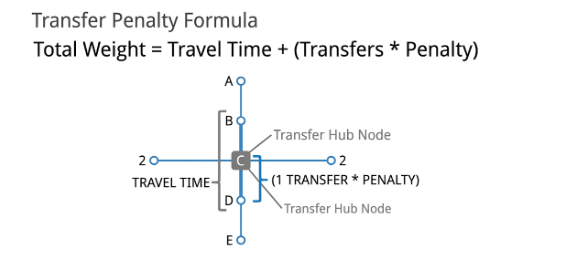
\includegraphics[width=0.68\textwidth]{Figures/Cap3/PenalizacionTransferencia.png}
    \caption[Diagrama del indicador de Penalización por Transferencia $W_{s,h}$]{
Nodo de transferencia con la descomposición del peso total en sus componentes
    de tiempo de caminata y espera.}
    \label{fig:indicador-W}
    \fuentefigura{Elaboración propia con base en \citet{allauca2023}.}
\end{figure}


\subsubsection{Nota Metodológica sobre Fuentes de Datos}

El uso de horarios \gtfs{} estáticos para estimar $T_{\text{wait}}$ introduce un
sesgo conocido: los datos estandarizados representan únicamente horarios
planificados, no tiempos reales de operación. \citet{fortin2016innovative}
reconocen esta limitación y señalan que los horarios inscritos pueden ser
incorrectos debido a la congestión o a errores de codificación. Para mitigar
este sesgo, la variante dinámica de la penalización se calibrará mediante
peticiones automatizadas a la \textit{Google Maps Directions API} (modo
\texttt{transit}, con variación del parámetro \texttt{departure\_time}), que
utiliza datos de \textit{crowdsourcing} (GPS de teléfonos móviles) para devolver
tiempos de espera y caminata ajustados a condiciones históricas reales en
distintos cortes horarios.

\subsubsection{Proyección Geográfica al Grafo: el Concepto de \termino{Snapping}}
\label{subsubsec:snapping}

Los indicadores $T$ y $W_{s,h}$ se calculan sobre nodos del grafo, pero los
datos de entrada ---paradas GTFS y puntos de transbordo--- son coordenadas
geográficas que rara vez coinciden con exactitud con algún nodo de la red OSM.
El \termino{snapping} resuelve esa discrepancia: para cada punto $p$ con
coordenadas $(lat, lon)$, la operación identifica el nodo más cercano
$v^* \in \mathcal{V}$ del grafo y lo adopta como representante:

\begin{equation}
    v^* = \arg\min_{v \in \mathcal{V}}\; d\!\left(p,\, v\right)
    \label{eq:snapping}
\end{equation}

donde $d(p, v)$ es la distancia haversine entre el punto geográfico y el nodo
del grafo. Sin este paso, el cálculo de $T_{\text{walk}}(s, h)$ sería
indefinido: el algoritmo no sabría desde qué nodo computar la ruta peatonal
hacia el andén de destino. El snapping constituye así el puente entre la
representación matemática del grafo y la geografía urbana real de la red,
haciendo posible traducir coordenadas de campo en insumos del modelo
\citep{fortin2016innovative}.

\subsubsection{Ejemplo Práctico: \cdmx{} y Zona Metropolitana}

\textbf{Par de transferencia:} Pantitlán Línea 1 Metro $\to$ Pantitlán Línea 9
Metro.

\begin{table}[H]
    \centering
    \caption{Estimaciones del indicador $W_{s,h}$ en la transferencia Pantitlán L1--L9.}
    \label{tab:penalizacion}
    \begin{tabularx}{\textwidth}{X r r}
        \toprule
        \textbf{Componente} & \textbf{Valor estático} &
        \textbf{Valor dinámico (hora pico 8:00\,h)} \\
        \midrule
        $T_{\text{walk}}$ (caminata entre andenes) & 3 min & 5 min \\
        $T_{\text{wait}}$ (espera en andén L9) & 4.5 min & 7 min \\
        $W_{s,h}$ \textbf{total} & \textbf{7.5 min} & \textbf{12 min} \\
        \bottomrule
    \end{tabularx}
\end{table}

El modelado correcto de $W_{s,h}$ es condición necesaria para que el grafo
multimodal construido en el Objetivo Específico 1 (§
\ref{subsec:obj-especificos} ) refleje la experiencia real del usuario. Un
algoritmo que omita esta penalización subestimaría los tiempos de viaje en rutas
multimodales e invalidaría el diagnóstico del Objetivo Específico 2, donde la
comparación entre escenarios descansa sobre la fidelidad del modelo de costos.
